\chapter{Human transcriptome and other layers of genomic information}\label{ch:integration}

\begin{quotation}
  \emph{The way to deal with the problem of big data is to beat it
    senseless with other big data.}
\begin{flushright}
J. Quackenbush (2006) %\cite{Eisenstein06b}
\end{flushright}
\end{quotation}


This chapter presents the third main contribution of the thesis,
computational strategies to integrate measurements of human
transcriptome to other layers of genomic information.  Genomic,
transcriptomic, proteomic, epigenomic and other sources of measurement
data characterize different aspects of genome organization
\citep{Hawkins2010, Montaner2010, Sara2010}; any single source
provides only a limited view to the cellular system. Understanding
functional organization of the genome and ultimately the cell function
requires integration of data from the various levels of genome
organization and modeling of their dynamical interplay.  Such an
holistic approach, which is also called {\it systems biology}, is a
key to understanding living organisms, which are ``rich in emergent
properties because forever new groups of properties emerge at every
level of integration'' \citep{Mayr04}. Combining evidence across
multiple sources can help to discover functional mechanisms and
interactions, which are not seen in the individual data sets, and to
increase statistical power in noisy and incomplete high-throughput
experiments \citep{Huttenhower2010, Reed2006}.

Integration of heterogeneous genomic data comes with a variety of
technical and methodological challenges \citep{Hwang05,
  Troyanskaya05}, and the particular modeling approaches vary
according to the analysis task and particular properties of the
investigated measurement sources.  Integrative studies have been
limited by poor availability of co-occurring genomic observations, but
suitable data sets are now becoming increasingly available in both
in-house and public biomedical data repositories \citep{tcga08}.  New
observations highlight the need for novel, integrative approaches in
functional genomics \citep{Coe08}. Recent studies have proposed for
instance methods to integrate epigenetic modifications
\citep{Sadikovic2008}, micro-RNA \citep{Qin2008}, transcription factor
binding \citep{Savage2010}, as well as protein expression
\citep{Johnson2008}.  Given the complex stochastic nature of
biological systems, computational efficiency, robustness against
uncertainty and interpretability of the results are key issues. Prior
information of biological systems is often incomplete, and subject to
high levels of uncontrolled variation and complex interdependencies
between different parts of the cellular system \citep{Troyanskaya05}.
These issues emphasize the need for principled approaches requiring
minimal prior knowledge about the data, as well as minimal model
fitting procedures. Section~\ref{sec:traditionaldep} gives an overview
of the standard models for high-throughput data integration methods,
which have close connections to the modeling approaches developed in
this work.

\section{Standard approaches for genomic data integration}\label{sec:traditionaldep}

The integrative approaches can be roughly classified in three
categories: methods that (i) combine statistical evidence across
related studies in order to obtain more accurate inferences of target
variables, (ii) utilize side information in order to guide the
analysis of a single, primary data source, and (iii) detect and
characterize dependencies between the measurement sources in order to
discover new functional connections between the different layers of
genomic information. The contributions in Chapters~\ref{ch:preproc}
and~\ref{ch:atlases} are associated with the first two categories; the
contributions presented in this chapter, the regularized dependency
detection framework of Publication~\ref{MLSP}, and associative
clustering of Publications~\ref{ECML} and~\ref{AC}, belong to the
third category.



\subsection{Combining statistical evidence}

The first general category of methods for genomic data integration
consists of approaches where evidence across similar studies is
combined to increase statistical power, for instance by comparing and
integrating data from independent microarray experiments targeted at
studying the same disease. In Publications~\ref{RPA} and~\ref{NR},
joint analysis of a large number of commensurable microarray
experiments, where the observed data is directly comparable between
the arrays, helps to increase statistical power and to reveal weak,
shared signals in the data that can not be detected in more restricted
experimental setups and smaller datasets. 

However, the related observations are often not directly comparable,
and further methodological tools are needed for integration. {\it
Meta-analysis} provides tools for such analysis
\citep{Ramasamy08b}. Meta-analysis forms part of the microarray
analysis procedure introduced in Publication~\ref{PECA}, where methods
to integrate related microarray measurements across different array
platforms are developed. Meta-analysis emphasizes shared effects
between the studies over statistical significance in individual
experiments. In its standard form, meta-analysis assumes that each
individual study measures the same target variable with varying levels
of noise. The analysis starts from identifying a measure of {\it
effect size} based on differences, means, or other summary statistics
of the observations such as the Hedges' g, used in
Publication~\ref{PECA}. Weighted averaging of the effect sizes
provides the final, combined result. Weighting accounts for
differences in reliability of the individual studies, for instance by
emphasizing studies with large sample size, or low measurement
variance. Averaging is expected to yield more accurate estimates of
the target variable than individual studies. This can be particularly
useful when several studies with small sample sizes are available for
instance from different laboratories, which is a common setting in
microarray analysis context, where the data sets produced by
individual laboratories are routinely deposited to shared community
databases. Ultimately, the quality of meta-analysis results rests on
the quality of the individual studies. Modeling choices, such as the
choice of the effect size measure and included studies will affect the
analysis outcome.

{\it Kernel methods} \citep[see e.g.][]{Scholkopf02} provide another
widely used approach for integrating statistical evidence across
multiple, potentially heterogeneous measurement sources. Kernel
methods operate on similarity matrices, and provide a natural
framework for combining statistical evidence to detect similarity and
patterns that are supported by multiple observations. The modeling
framework also allows for efficient modeling of nonlinear feature
spaces.

{\it Multi-task learning} refers to a class of approaches where
multiple, related modeling tasks are solved simultaneously by
combining statistical power across the related tasks. A typical task
is to improve the accuracy of individual classifiers by taking
advantage of the potential dependencies between them \citep[see
e.g.][]{Caruana97}.


\subsection{Role of side information}

The second category of approaches for genomic data integration
consists of methods that are asymmetric by nature; integration is used
to support the analysis of one, primary data source. Side information
can be used, for instance, to limit the search space and to focus the
analysis to avoid overfitting, speed up computation, as well as to
obtain potentially more sensitive and accurate findings \citep[see
e.g.][]{Eisenstein06}. One strategy is to impose hard constraints on
the model, or model family, based on side information to target
specific research questions. In gene expression context, functional
classifications or known interactions between the genes can be used to
constrain the analysis \citep{Goeman07, Ulitsky09}. In factor analysis
and mixed effect models, clinical annotations of the samples help to
focus the modeling on particular conditions \citep[see
e.g.][]{Carvalho08}. Hard constraints rely heavily on the accuracy of
side information. Soft, or probabilistic approaches can take the
uncertainty in side information into account, but they are
computationally more demanding. Examples of such methods in the
context of transcriptome analysis include for instance the supervised
biclustering models, such as cMonkey and modified SAMBA, as well as
other methods that guide the analysis with additional information of
genes and regulatory mechanisms, such as transcription factor binding
\citep{Reiss06, Savage2010, Tanay04}. Publication~\ref{NR} uses gene
interaction network as a hard constraint for modeling transcriptional
co-regulation of the genes, but the condition-specific responses of
the detected gene groups are identified in an unsupervised manner.

A complementary approach for utilizing side information of the
experiments is provided by {\it multi-way learning}. A classical
example is the analysis of variance (ANOVA), where a single data set
is modeled by decomposing it into a set of basic, underlying effects,
which characterize the data optimally. The effects are associated with
multiple, potentially overlapping attributes of the measurement
samples, such as disease state, gender and age, which are known prior
to the analysis. Taking such prior knowledge of systematic variation
between the samples into account helps to increase modeling power and
can reveal the attribute-specific effects. An interesting subtask is
to model the interactions between the attributes, so-called {\it
interaction effects}. These are manifested only with particular
combinations of attributes, and indicate dependency between the
attributes. For instance, simultaneous cigarette smoking and asbestos
exposure will considerably increase the risk of lung cancer, compared
to any of the two risk factors alone \citep[see
e.g.][]{Nymark07}. {\it Factor analysis} is a closely related approach
where the attributes, also called {\it factors}, are not given but
instead estimated from the data. {\it Mixed effect models} combine the
supervised and unsupervised approaches by incorporating both {\it
fixed} and {\it random effects} in the model, corresponding to the
known and latent attributes, respectively \citep[see
e.g.][]{Carvalho08}. The standard factorization approaches for
individual data sets are related to the dependency-seeking approaches
in Publications~\ref{MLSP}-\ref{AC}, where co-occurring data sources
are decomposed in an unsupervised manner into components that are
maximally informative of the components in the other data set. 

\subsection{Modeling of mutual dependency}

Symmetric models for dependency detection form the third main category
of methods for genomic data integration, as well as the main topic of
this chapter. Dependency modeling is used to distinguish the {\it
shared} signal from {\it dataset-specific} variation. The shared
effects are informative of the commonalities and interactions between
the observations, and are often the main focus of interest in
integrative analysis. This motivates the development of methods that
can allocate computational resources efficiently to modeling of the
shared features and interactions.

{\it Multi-view learning} is a general category of approaches for
symmetric dependency modeling tasks. In multi-view learning, multiple
measurement sources are available, and each source is considered as a
different view on the same objects. The task is to enhance modeling
performance by combining the complementary views. A classical example
of such a model is canonical correlation analysis
\citep{Hotelling36}. Related approaches that have recently been applied
in functional genomics include for instance probabilistic variants of
meta-analysis \citep{Choi07, Conlon07}, generalized singular value
decomposition \citep[see e.g.][]{Alter03, Berger06} and simultaneous
non-negative matrix factorization \citep{Badea08}.

The dependency modeling approaches in this thesis make an explicit
distinction between statistical representation of data and the
modeling task.  Let us denote the representations of two co-occurring
multivariate observations, $\x$ and $\y$, with $f_x(\x)$ and
$f_y(\y)$, respectively. The selected representations depend on the
application task. The representation can be for instance used to
perform feature selection as in {\it canonical correlation analysis
(CCA)} \citet{Hotelling36}, capture nonlinear features in the data as
in kernelized versions of CCA \citep[see e.g.][]{Yamanishi03}, or
partition the data as in information bottleneck \citep{Friedman01} and
associative clustering (Publications~\ref{ECML}-\ref{AC}). {\it
Statistical independence} of the representations implies that their
joint probability density can be decomposed as \(p(f_x(\x), f_y(\y)) =
p(f_x(\x))p(f_y(\y))\). Deviations from this assumption indicate
statistical dependency. The representations can have a flexible
parametric form which can be optimized by the dependency modeling
algorithms to identify dependency structure in the data.

Recent examples of such dependency-maximizing methods include
probabilistic canonical correlation analysis \citep{Bach05}, which has
close theoretical connection to the regularized models introduced in
Publication~\ref{MLSP}, and the associative clustering principle
introduced in Publications~\ref{ECML}-\ref{AC}. Canonical
correlations and contingency table analysis form the methodological
background for the contributions in Publications~\ref{MLSP}-\ref{AC}.
In the remainder of this section these two standard approaches for
dependency detection are considered more closely.

\subsubsection{Classical and probabilistic canonical correlation analysis}

Canonical correlation analysis (CCA) is a classical method for
detecting linear dependencies between two multivariate random
variables \citep{Hotelling36}. While ordinary correlation
characterizes the association strength between two vectors with paired
scalar observations, CCA assumes paired vectorial values, and
generalizes correlation to multidimensional sources by searching for
maximally correlating low-dimensional representation of the two
sources, defined by linear projections \(\X\vx, \Y\vy\). Multiple
projection components can be obtained iteratively, by finding the most
correlating projection first, and then consecutively the next ones
after removing the dependencies explained by the previous CCA
components; the lower-dimensional representations are defined by
projections to linear hyperplanes. The model can be formulated as a
generalized eigenvalue problem that has an analytical solution with
two useful properties: the result is invariant to linear
transformations of the data, and the solution for any fixed number of
components maximizes mutual information between the projections for
Gaussian data \citep{Kullback59, Bach02}. Extensions of the classical
CCA include generalizations to multiple data sources
\citep{Kettenring71, Bach02}, regularized solutions with non-negative
and sparse projections \citep{Sigg07, Archambeau08, Witten09}, and
non-linear extensions, for instance with kernel methods \citep{Bach02,
Yamanishi03}. Direct optimization of correlations in the classical CCA
provides an efficient way to detect dependencies between data sources,
but it lacks an explicit model to deal with the uncertainty in the
data and model parameters.

Recently, the classical CCA was shown to correspond to the ML solution
of a particular generative model where the two data sets are assumed
to stem from a shared Gaussian latent variable \(\z\) and normally
distributed data-set-specific noise \citep{Bach05}. Using linear
assumptions, the model is formally defined as

\begin{flalign}\label{eq:genmodel}
     \left\{
   \begin{array}{cl}
	\x &\sim \Wx \z + \Epsx\\
	\y &\sim \Wy \z + \Epsy.
  \end{array}
\right.
\end{flalign}

\noindent The manifestation of the shared signal in each data set can
be different. This is parameterized by \(\W_x\) and \(\W_y\).
Assuming a standard Gaussian model for the shared latent variable,
\(\z \sim \N(\0,\I)\) and data set-specific effects where \(\Epsx \sim
\N(\0, \Psi_x)\) (and respectively for \(\y\)), the
correlation-maximizing projections of the traditional CCA introduced
in Section~\ref{sec:traditionaldep} can be retrieved from the ML
solution of the model \citep{Archambeau06, Bach05}. The model
decomposes the observed co-occurring data sets into {\it shared} and
{\it data set-specific} components based on explicit modeling
assumptions (Figure~\ref{fig:modelpic}). The dataset-specific effects
can also be described in terms of latent variables as \(\Epsx =
\B_x\z_x\) and \(\Epsy = \B_y\z_y\), allowing the construction of more
detailed models for the dataset-specific effects \citep{Klami08}. The
shared signal \(\z\) is treated as a latent variable and marginalized
out in the model, providing the marginal likelihood for the
observations:

\begin{equation}\label{eq:ccalikelihood}
    p(\X,\Y|\W,\Psi) = \int p(\X, \Y|\Z, \W, \Psi)p(\Z) d\Z,
\end{equation}

\noindent where \(\Psi\) denotes the block-diagonal matrix of
\(\Psi_x\), \(\Psi_y\), and \(\W = [\W_x; \W_y]\).  The probabilistic
formulation of CCA has opened up a way to new probabilistic extensions
that can treat the modeling assumptions and uncertainties in the data
in a more explicit and robust manner \citep{Archambeau06, Klami08,
Klami10uai}.

The general formulation provides a flexible modeling framework, where
different modeling assumptions can be used to adapt the models in
different applications. The connection to classical CCA assumes full
covariances for the dataset-specific effects. Simpler models for the
dataset-specific effects will not distinguish between the shared and
marginal effects as effectively, but they have fewer model parameters
that can potentially reduce overlearning and speed up computation.  It
is also possible to tune the dimensionality of the shared latent
signal. Learning of lower-dimensional models can be faster and
potentially less prone to overfitting. Interpretation of simpler
models is also more straightforward in many applications. The
probabilistic formulation allows rigorous treatment of uncertainties
in the data and model parameters also with small sample sizes that are
common in biomedical studies, and allows the incorporation of prior
information through Bayesian priors, as in the regularized dependency
detection framework introduced in Publication~\ref{MLSP}.


\begin{figure}[ht!]
\centering{ 
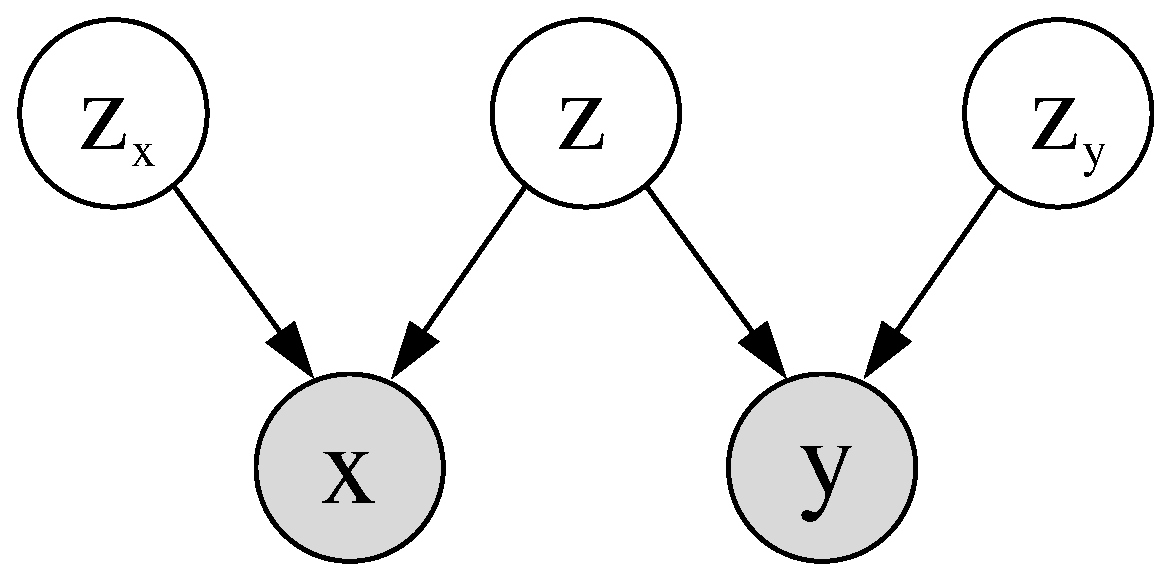
\includegraphics[width=.4\textwidth]{pic/depmodel.eps}
}
\caption{A graphical representation of the generative shared latent
  variable model in Equation~(\ref{eq:genmodel}). The latent source
  $\z$ is shared by observations $\x$ and $\y$. The other effects that
  are specific to each observation are characterized by $\z_x$ and
  $\z_y$, respectively. Gray shading indicates observed variables.}
\label{fig:modelpic}
\end{figure}


\subsubsection{Contingency table analysis}

Contingency table analysis is a classical approach used to study
associations between co-occurring categorical observations.  The
co-occurrences are represented by cross-tabulating them on a {\it
contingency table}, the rows and columns of which correspond to the
first and second set of features, respectively. Various tests are
available for measuring dependency between the rows and columns of the
table \citet{Yates34, Agresti92}, including the classical Fisher test
\citep{Fisher34}, a standard tool for measuring statistical enrichment
of functional categories in gene cluster analysis
\citep{Hosack03}. While the classical contingency table analysis is
used to measure dependency between co-occurring variables, more recent
approaches use contingency tables to derive objective functions for
dependency exploration tasks. The associative clustering principle
introduced in Publications~\ref{ECML}-\ref{AC} is an example of such
approach.

Other approaches that use contingency table dependencies as objective
functions include the {\it information bottleneck (IB)} principle
\citep{Tishby99} and {\it discriminative clustering (DC)}
\citep{Sinkkonen02ecml, Kaski05nc}. These are asymmetric,
dependency-seeking approaches that can be used to discover cluster
structure in a primary data such that it is maximally informative of
another, discrete auxiliary variable. The dependency is represented on
a contingency table, and maximization of contingency table
dependencies provides the objective function for clustering. While the
standard IB operates on discrete data, DC is used to discover cluster
structure in continuous-valued data. The two approaches also employ
different objective functions. In classical IB, a discrete variable
$\Xcal$ is clustered in such a way that the cluster assignments become
maximally informative of another discrete variable $\Ycal$. The
complexity of the cluster assignments is controlled by minimizing the
mutual information between the cluster indices and the original
variables. The task is to find a partitioning $\tilde{\X}$ that
minimizes the cost \(\L(p(\tilde{\X}|\X)) = I(\tilde{\X}; \X) - \beta
I(\tilde{\X}; \Y),\) where $\beta$ controls clustering resolution. In
DC, mutual information is replaced by a Bayes factor between the two
hypotheses of dependent and independent margins. The Bayes factor is
asymptotically consistent with mutual information, but provides an
unbiased estimate for limited sample size \citep[see
e.g.][]{Sinkkonen05tr}. The standard information bottleneck and
discriminative clustering are asymmetric methods that treat one of the
data sources as the primary target of analysis.

In contrast, the dependency maximization approaches considered in this
thesis, the associative clustering (AC) and regularized versions of
canonical correlation analysis are symmetric and they operate
exclusively on continuous-valued data.  CCA is not based on
contingency table analysis, but it has close connections to the
Gaussian IB \citep{Chechik05} that seeks maximal dependency between
two sets of normally distributed variables. The Gaussian IB retrieves
the same subspace as CCA for one of the data sets. However, in
contrast to the symmetric CCA model, Gaussian IB is a directed method
that finds dependency-maximizing projections for only one of the two
data sets.  The second dependency detection approach considered in
this thesis, the associative clustering, is particularly related to
the symmetric IB that finds two sets of clusters, one for each
variable, which are optimally compressed presentations of the original
data, and at the same time maximally informative of each other
\citep{Friedman01}. While the objective function in IB is derived from
mutual information, AC uses the Bayes factor as an objective function
in a similar manner as it is used in the asymmetric discriminative
clustering. Another key difference is that while the symmetric IB
operates on discrete data, AC employs contingency table analysis in
order to discover cluster structure in continuous-valued data spaces.








\section{Regularized dependency detection}\label{sec:pairwise}

Standard unsupervised methods for dependency detection, such as the
canonical correlation analysis or the symmetric information bottleneck,
seek maximal dependency between two data sets with minimal assumptions
about the dependencies. The unconstrained models involve high degrees
of freedom when applied to high-dimensional genomic observations. Such
flexibility can easily lead to overfitting, which is even worse for
more flexible nonparametric or nonlinear, kernel-based dependency
discovery methods.  Several ways to regularize the solution have been
suggested to overcome associated problems, for instance by imposing
sparsity constraints on the solution space \citep{Bie03, Vinod76}.

In many applications prior information of the dependencies is
available, or particular types of dependency are relevant for the
analysis task. Such prior information can be used to reduce the
degrees of freedom in the model, and to regularize dependency
detection. In the cancer gene discovery application of
Publication~\ref{MLSP}, DNA mutations are systematically correlated
with transcriptional activity of the genes within the affected region,
and identification of such regions is a biomedically relevant research
task. Prior knowledge of chromosomal distances between the
observations can improve the detection of the relevant spatial
dependencies. However, principled approaches to incorporate such prior
information in dependency modeling have been
missing. Publication~\ref{MLSP} introduces regularized models for
dependency detection based on classical canonical correlation analysis
\citep{Hotelling36} and its probabilistic formulation
\citep{Bach05}. The models are extended by incorporating appropriate
prior terms, which are then used to reduce the degrees of freedom
based on prior biological knowledge.


\subsubsection{Correlation-based variant}

In order to introduce the regularized dependency detection framework
of Publication~\ref{MLSP}, let us start by considering regularization
of the classical correlation-based CCA. This searches for arbitrary
linear projection vectors \(\vx, \vy\) that maximize the correlation
between the projections of the data sets \(\X, \Y\). Multiple
projection components can be obtained iteratively, by finding the most
correlating projection first, and then consecutively the next ones
after removing the dependencies explained by the previous CCA
components. The procedure will identify maximally dependent linear
subspaces of the investigated data sets. To regularize the solution,
Publication~\ref{MLSP} couples the projections through a
transformation matrix \(\T\) in such a way that \(\vy = \T \vx\). With
a completely unconstrained \(\T\) the model reduces to the classical
unconstrained CCA; suitable constraints on can be used to regularize
dependency detection.

To enforce regularization one could for instance prefer solutions for
\(\T\) that are close to a given transformation matrix, \(\T \sim
\M\), or impose more general constraints on the structure of the
transformation matrix that would prefer particular rotational or other
linear relationships. Suitable constraints depend on the particular
applications; the solutions can be made to prefer particular types of
dependency in a soft manner by appropriate penalty terms. In
Publication~\ref{MLSP} the completely unconstrained CCA model has been
compared with a fully regularized model with \(\T = \I\); this encodes
the biological assumption that probes with small chromosomal distances
tend to capture more similar signal between gene expression and copy
number measurements than probes with a larger chromosomal distance;
the projection vectors characterize this relationship, and are
therefore expected to have similar form, \(\vx \sim \vy\). Utilization
of other, more general constraints in related data integration tasks
provides a promising topic for future studies.

The correlation-based treatment provides an intuitive and easily
implementable formulation for regularized dependency
detection. However, it lacks an explicit model for the shared and
data-specific effects, and it is likely that some of the
dataset-specific effects are captured by the correlation-maximizing
projections. This is suboptimal for characterizing the shared effects,
and motivates the probabilistic treatment.

\subsubsection{Probabilistic dependency detection with similarity constraints}

The probabilistic approach for regularized dependency detection in
Publication~\ref{MLSP} is based on an explicit model of the
data-generating process formulated in Equation~(\ref{eq:genmodel}). In
this model, the transformation matrices \(\W_x\), \(\W_y\) specify how
the shared latent variable \(\Z\) is manifested in each data set
\(\X\), \(\Y\), respectively. In the standard model, the relationship
between the transformation matrices is not constrained, and the
algorithm searches for arbitrary linear transformations that maximize
the likelihood of the observations in
Equation~(\ref{eq:ccalikelihood}). The probabilistic formulation opens
up possibilities to guide dependency search through Bayesian priors.

In Publication~\ref{MLSP}, the standard probabilistic CCA model is
extended by incorporating additional prior terms that regularize the
relationship by reparameterizing the transformation matrices as \(\W_y
= \T\W_x\), and setting a prior on \(\T\). The treatment is analogous
to the correlation-based variant, but now the transformation matrices
operate on the latent components, rather than the observations. This
allows to distinguish the shared and dataset-specific effects more
explicitly in the model. The task is then to learn the optimal
parameter matrix \(\W = [\Wx; \Wy]\), given the constraint \(\W_y =
\T\W_x\). The Bayes' rule gives the model likelihood

\begin{equation}\label{eq:ccafull}
  p(\X, \Y, \W, \Psib) \sim p(\X, \Y | \W, \Psib) p(\W, \Psib).
\end{equation}

\noindent The likelihood term \(p(\X, \Y | \W, \Psib)\) can be
calculated based on the model in Equation~(\ref{eq:genmodel}). This
defines the objective function for standard probabilistic CCA, which
implicitly assumes a flat prior \(p(\W, \Psib) \sim 1\) for the model
parameters. The formulation in Equation~(\ref{eq:ccafull}) makes the
choice of the prior explicit, allowing modifications on the prior
term. To obtain a tractable prior, let us assume that the prior
factorizes as \(p(\W, \Psib) = p( \W ) p( \Psib )\). The first term
can be further decomposed as \(p(\W) \sim p(\W_x) p(\T)\), assuming
independent priors for \(\W_x\) and \(\T\). A convenient and tractable
prior for \(\T\) is provided by the matrix normal
distribution:\footnote{\(\Nm(\T | \M, \U, \Vb) \sim
  exp\left(-\frac{1}{2} Tr\{\U^{-1}(\T-\M)\Vb^{-1}(\T -
    \M)^T\}\right)\) where \(\M\) is the mean matrix, and \(\U\) and
  \(\Vb\) denote row and column covariances, respectively.}

\begin{equation}\label{eq:Nm}
  p(\T) = \Nm(\T | \M, \U, \Vb).
\end{equation}

\noindent For computational simplicity, let us assume independent rows
and columns with \(\U = \Vb = \sigma_T \I\). The mean matrix \(\M\)
can be used to emphasize certain types of dependency between \(\Wx\)
and \(\Wy\). Assuming uninformative, flat priors \(p(\Wx) \sim 1\) and
\(p(\Psib) \sim 1\), as in the standard probabilistic CCA model, and
denoting \(\bSigma = \W\W^T + \Psib \), the negative log-likelihood of
the model is

\begin{equation}\label{eq:simccacost}
  -logp(\X, \Y, \W, \Psib) \sim log|\bSigma| + Tr \bSigma^{-1} \tilde{\bSigma} +
  \frac{\parallel \T - \M \parallel_{F}^2}{2\sigt}.
\end{equation}

\noindent This is the objective function to minimize. Note that this
has the same form as the objective function of the standard
probabilistic CCA, except the additional penalty term
\(\frac{\parallel \T - \M \parallel_{F}^2}{2\sigt}\) arising from the
prior \(p(\T)\). This yields the cost function employed in
Publication~\ref{MLSP}. In our cancer gene discovery application the
choice \(\M = \I\) is used to encode the biological prior constrain
\(\T \approx \I\), which states that the observations with a small
chromosomal distance should on average show similar responses in the
integrated data sets, i.e., \(\Wx \approx \Wy\). The regularization
strength can be tuned with \(\sigt\). A fully regularized model is
obtained with \(\sigt \rightarrow 0\). When \(\sigt \rightarrow
\infty\), $\W_x$ and $\W_y$ become independent {\it a priori},
yielding the ordinary probabilistic CCA. The \(\sigt\) can be used to
regularize the solution between these two extremes. Note that it is
possible to incorporate also other types of prior information
concerning the dependencies into the model through \(p(\T)\).

The model parameters \(\W\), \(\Psib\) are estimated with the EM
algorithm. The regularized version is not analytically tractable with
respect to \(\W\) in the general case, but can be optimized with
standard gradient-based optimization techniques. Special cases of the
model have analytical solutions, which can speed up the model fitting
procedure. In particular, the fully regularized and unconstrained
models, obtained with \(\sigt = 0\) and \(\sigt = \infty\)
respectively, have closed-form solutions for \(\W\). Note that the
current formulation assumes that the regularization parameters \(\M,
\sigt\) are defined prior to the analysis. Alternatively, these
parameters could be optimized based on external criteria, such as
cancer gene detection performance in our application, or learned from
the data in a fully Bayesian treatment these parameters would be
treated as latent variables. Incorporation of additional prior
information of the data set-specific effects through priors on
\(\W_x\) and \(\Psib\) provides promising lines for further work.

\subsection{Cancer gene discovery with dependency detection}

The regularized models provide a principled framework for studying
associations between transcriptional activity and other regulatory
layers of the genome. In Publication~\ref{MLSP}, the models are used
to investigate cancer mechanisms. DNA copy number changes are a key
mechanism for cancer, and integration of copy number information with
mRNA expression measurements can reveal functional effects of the
mutations. While causation may be difficult to grasp, study of the
dependencies can help to identify functionally active mutations, and
to provide candidate biomarkers with potential diagnostic, prognostic
and clinical impact in cancer studies.

The modeling task in the cancer gene discovery application of
Publication~\ref{MLSP} is to identify chromosomal regions that show
exceptionally high levels of dependency between gene copy number and
transcriptional levels.  The model is used to detect dependency within
local chromosomal regions that are then compared in order to identify
the exceptional regions. The dependency is quantified within a given
region by comparing the strength of shared and data set-specific
signal. High scores indicate regions where the shared signal is
particularly high relative to the data-set-specific effects.  A
sliding-window approach is used to screen the genome for
dependencies. The regions are defined by the \(d\) closest probes
around each gene. Then the dimensionality of the models stays
constant, which allows direct comparison of the dependency measures
between the regions without additional adjustment terms that would be
otherwise needed to compensate for differences in model complexity.

Prior information of the dependencies is used to regularize cancer
gene detection. Chromosomal gains and losses are likely to be
positively correlated with the expression levels of the affected genes
within the same chromosomal region or its close proximity; copy number
gain is likely to increase the expression of the associated genes
whereas deletion will block gene expression.  The prior information is
encoded in the model by setting \(\M = \I\) in the prior term
\(p(\T)\). This accounts for the expected positive correlations
between gene expression and copy number within the investigated
chromosomal region. Regularization based on such prior information is
shown to improve cancer gene detection performance in
Publication~\ref{MLSP}, where the regularized variants outperformed
the unconstrained models.

A genome-wide screen of 51 gastric cancer patients
\citep{Myllykangas08jc} reveals clear associations between DNA copy
number changes and transcriptional activity. The Figure~\ref{fig:17q}
illustrates dependency detection on chromosome arm 17q, where the
regularized model reveals high dependency between the two data sources
in a known cancer-associated region.  The regularized and
unconstrained models were compared in terms of receiver-operator
characteristics calculated by comparing the ordered gene list from the
dependency screen to an expert-curated list of known genes associated
with gastric cancer \citep{Myllykangas08jc}. A large proportion of the
most significant findings in the whole-genome analysis were known
cancer genes; the remaining findings with no known associations to
gastric cancer are promising candidates for further study.

Biomedical interpretation of the model parameters is also
straightforward. A ML estimate of the latent variable values \(\Z\)
characterizes the strength of the shared signal between DNA mutations
and transcriptional activity for each patient. This allows robust
identification of small, potentially unknown patient subgroups with
shared amplification effects. These would remain potentially
undetected when comparing patient groups defined based on existing
clinical annotations. The parameters in \(\W\) can downweigh signal
from poorly performing probes in each data set, or probes that measure
genes whose transcriptional levels are not functionally affected by
the copy number change. This provides tools to distinguish between
so-called {\it driver} mutations having functional effects from less
active {\it passenger} mutations, which is an important task in cancer
studies.  On the other hand, the model can combine statistical power
across the adjacent measurement probes, and it captures the strongest
shared signal in the two sets of observations. This is useful since
gene expression and copy number data are typically characterized by
high levels of biological and measurement variation and small sample
size.

\begin{figure}[ht!]
\centerline{
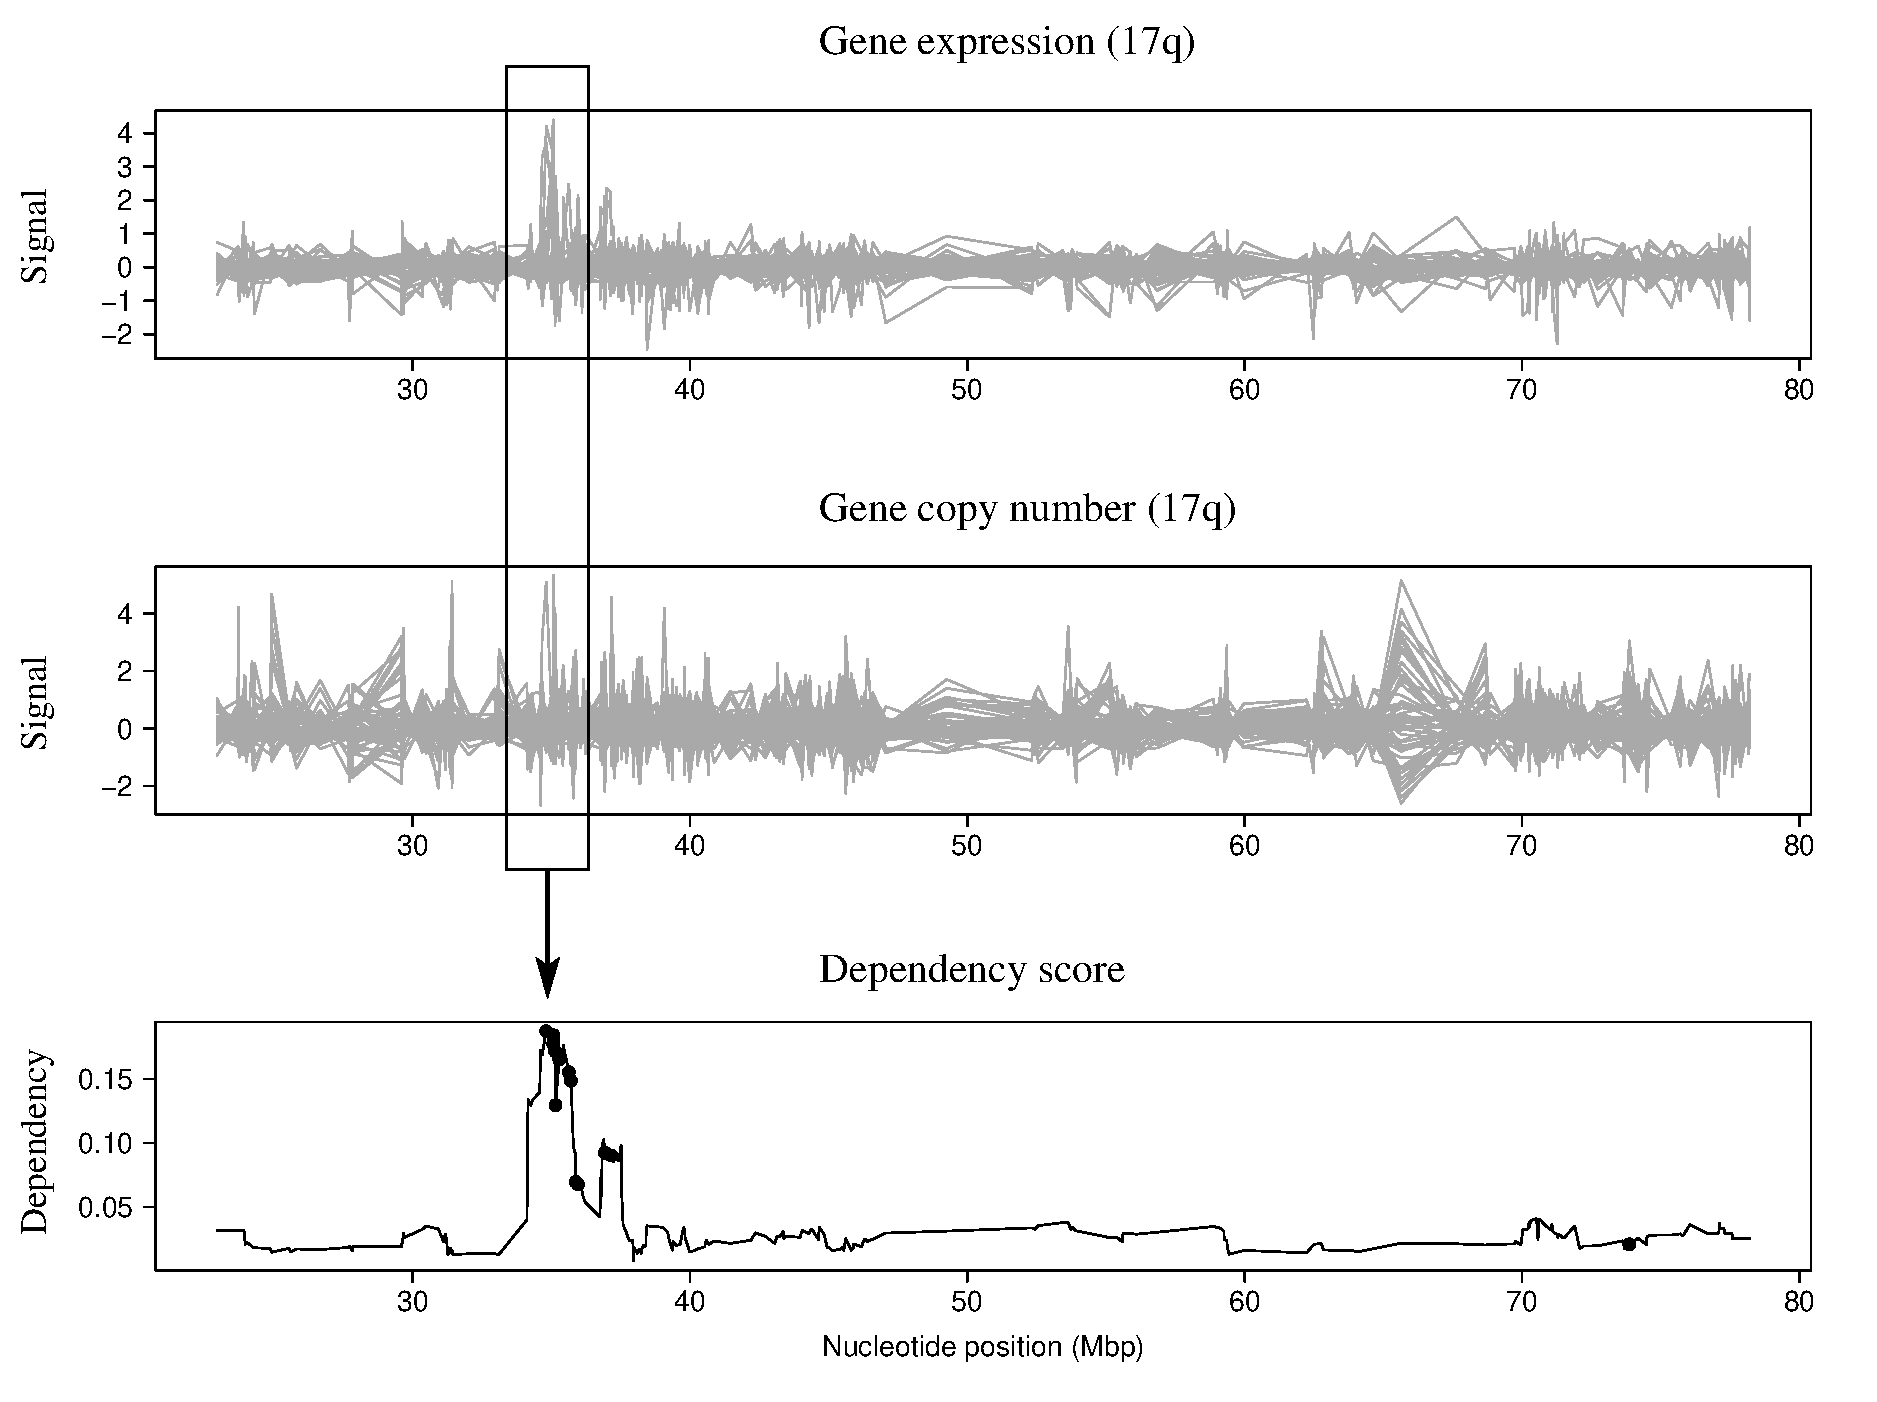
\includegraphics[width=1\textwidth]{pic/17q.eps}} 
\caption{Gene expression, copy number signal, and the dependency score
  along the chromosome arm 17q obtained with the regularized latent
  variable framework in Equation~\ref{eq:simccacost}. Known
  cancer-associated genes from an expert-curated list are marked with
  black dots.}
\label{fig:17q}
\end{figure}
% Produced with pic/chr17q.R + xfig

\subsubsection{Related approaches}

Integration of chromosomal aberrations and transcriptional activity is
an actively studied data integration task in functional genomics. The
first studies with standard statistical tests were carried out by
\citet{Hyman2002} and \citet{Phillips2001} when simultaneous
genome-wide observations of the two data sources had become available.
The modeling approaches utilized in this context can be roughly
classified in regression-based, correlation-based and latent variable
approaches. The regression-based models \citep{Adler2006, Bicciato09,
  Wieringen09} characterize alterations in gene expression levels
based on copy number observations with multivariate regression or
closely related models. The correlation-based approaches
\citep{Gonzalez2009, Schafer09, Soneson2010} provide symmetric models
for dependency detection, based on correlation and related statistical
models. Many of these methods also regularize the solutions, typically
based on sparsity constraints and non-negativity of the projections
\citep{LeCao2009, Waaijenborg2008, Witten09, Parkhomenko2009}. The
correlation-based approach in Publication~\ref{MLSP} introduces a
complementary approach for regularization that constrains the
relationship between subspaces where the correlations are
estimated. The latent variable models by \cite{Berger06, Shen09,
  Vaske2010}, and Publication~\ref{MLSP} are based on explicit
modeling assumptions concerning the data-generating processes. The
iCluster algorithm \citep{Shen09} is closely related to the latent
variable model considered in Publication~\ref{MLSP}. While our model
detects continuous dependencies, iCluster uses a discrete latent
variable to partition the samples into distinct subgroups.  The
iCluster model is regularized by sparsity constraints on \(\W\), while
we tune the relationship between \(\Wx\) and \(\Wy\). Moreover, the
model in Publication~\ref{MLSP} utilizes full covariance matrices to
model for the dataset-specific effects, whereas iCluster uses diagonal
covariances. The more detailed model for dataset-specific effects in
our model should help to distinguish the shared signal more
accurately. Other latent variable approaches include the iterative
method based on generalized singular-value decomposition
\citep{Berger06}, and the probabilistic factor graph model PARADIGM
\citep{Vaske2010}, which additionally utilizes pathway topology
information in the modeling.

Experimental comparison between the related integrative approaches can
be problematic since they target related, but different research
questions where the biological ground truth is often unknown.  For
instance, some methods utilize patient class information in order to
detect class-specific alterations \citep{Schafer09}, other methods
perform {\it de novo} class discovery \citep{Shen09}, provide tools
for gene prioritization \citep{Salari2010}, or guide the analysis with
additional functional information of the genes \citep{Vaske2010}. The
algorithms introduced in Publication~\ref{MLSP} are particularly
useful for gene prioritization and class discovery purposes, where the
target is to identify the most promising cancer gene candidates for
further validation, or to detect potentially novel cancer
subtypes. However, while an increasing number of methods are released
as conveniently accessible algorithmic tools \citep{Salari2010,
  Shen09, Schafer09, Witten09}, implementations of most models are not
available for comparison purposes. Open source implementations of the
dependency detection algorithms developed in this thesis have been
released to enhance transparency and reproducibility of the
computational experiments and to encourage further use of these models
\citep{Lahti10pint}.




\section{Associative clustering}

Functions of human genes are often studied indirectly, by studying
model organisms such as the mouse \citep{Davis04, Joyce06}. Orthologs
are genes in different species that originate from a single gene in
the last common ancestor of these species. Such genes have often
retained identical biological roles in the present-day organisms, and
are likely to share the function \citep{Fitch70}. Mutations in the
genomic DNA sequence are a key mechanism in evolution. Consequently,
DNA sequence similarity can provide hypotheses of gene function in
poorly annotated species. An exceptional level of conservation may
highlight critical physiological similarities between species, whereas
divergence can indicate significant evolutionary changes
\citep{Jordan05}. Investigating evolutionary conservation and
divergence will potentially lead to a deeper understanding of what
makes each species unique.  Evolutionary changes primarily target the
structure and sequence of genomic DNA. However, not all changes will
lead to phenotypic differences.  On the other hand, sequence
similarity is not a guarantee of functional similarity because small
changes in DNA can potentially have remarkable functional
implications.

Therefore, in addition to investigating {\it structural conservation}
of the genes at the sequence level, another level of investigation is
needed to study {\it functional conservation} of the genes and their
regulation, which is reflected at the transcriptome \citep{Jimenez02,
  Jordan05}. Transcriptional regulation of the genes is a key
regulatory mechanism that can have remarkable phenotypic consequences
in highly modular cell-biological systems \citep{Hartwell99} even when
the original function of the regulated genes would remain intact.

Systematic comparison of transcriptional activity between different
species would provide a straightforward strategy for investigating
conservation of gene regulation \citep{Bergmann04, Enard02, Zhou04}.
However, direct comparison of individual genes between species may not
be optimal for discovering subtle and complex dependency structures.
The associative clustering principle (AC), introduced in
Publications~\ref{ECML}-\ref{AC}, provides a framework for detecting
groups of orthologous genes with exceptional levels of conservation
and divergence in transcriptional activity between two species. While
standard dependency detection methods for continuous data, such as the
generalized singular value decomposition \citep[see e.g.][]{Alter03}
or canonical correlation analysis \citep{Hotelling36} detect global
linear dependencies between observations, AC searches for dependent,
local groupings to reveal gene groups with exceptional levels of
conservation and divergence in transcriptional activity.  The model is
free of particular distributional assumptions about the data, which
helps to allocate modeling resources to detecting dependent subgroups
when variation within each group is less relevant for the analysis.
The remainder of this section provides an overview of the associative
clustering principle and its application to studying evolutionary
divergence between species.

\begin{figure}[t]
\label{fig:acprinciple}
\centerline{
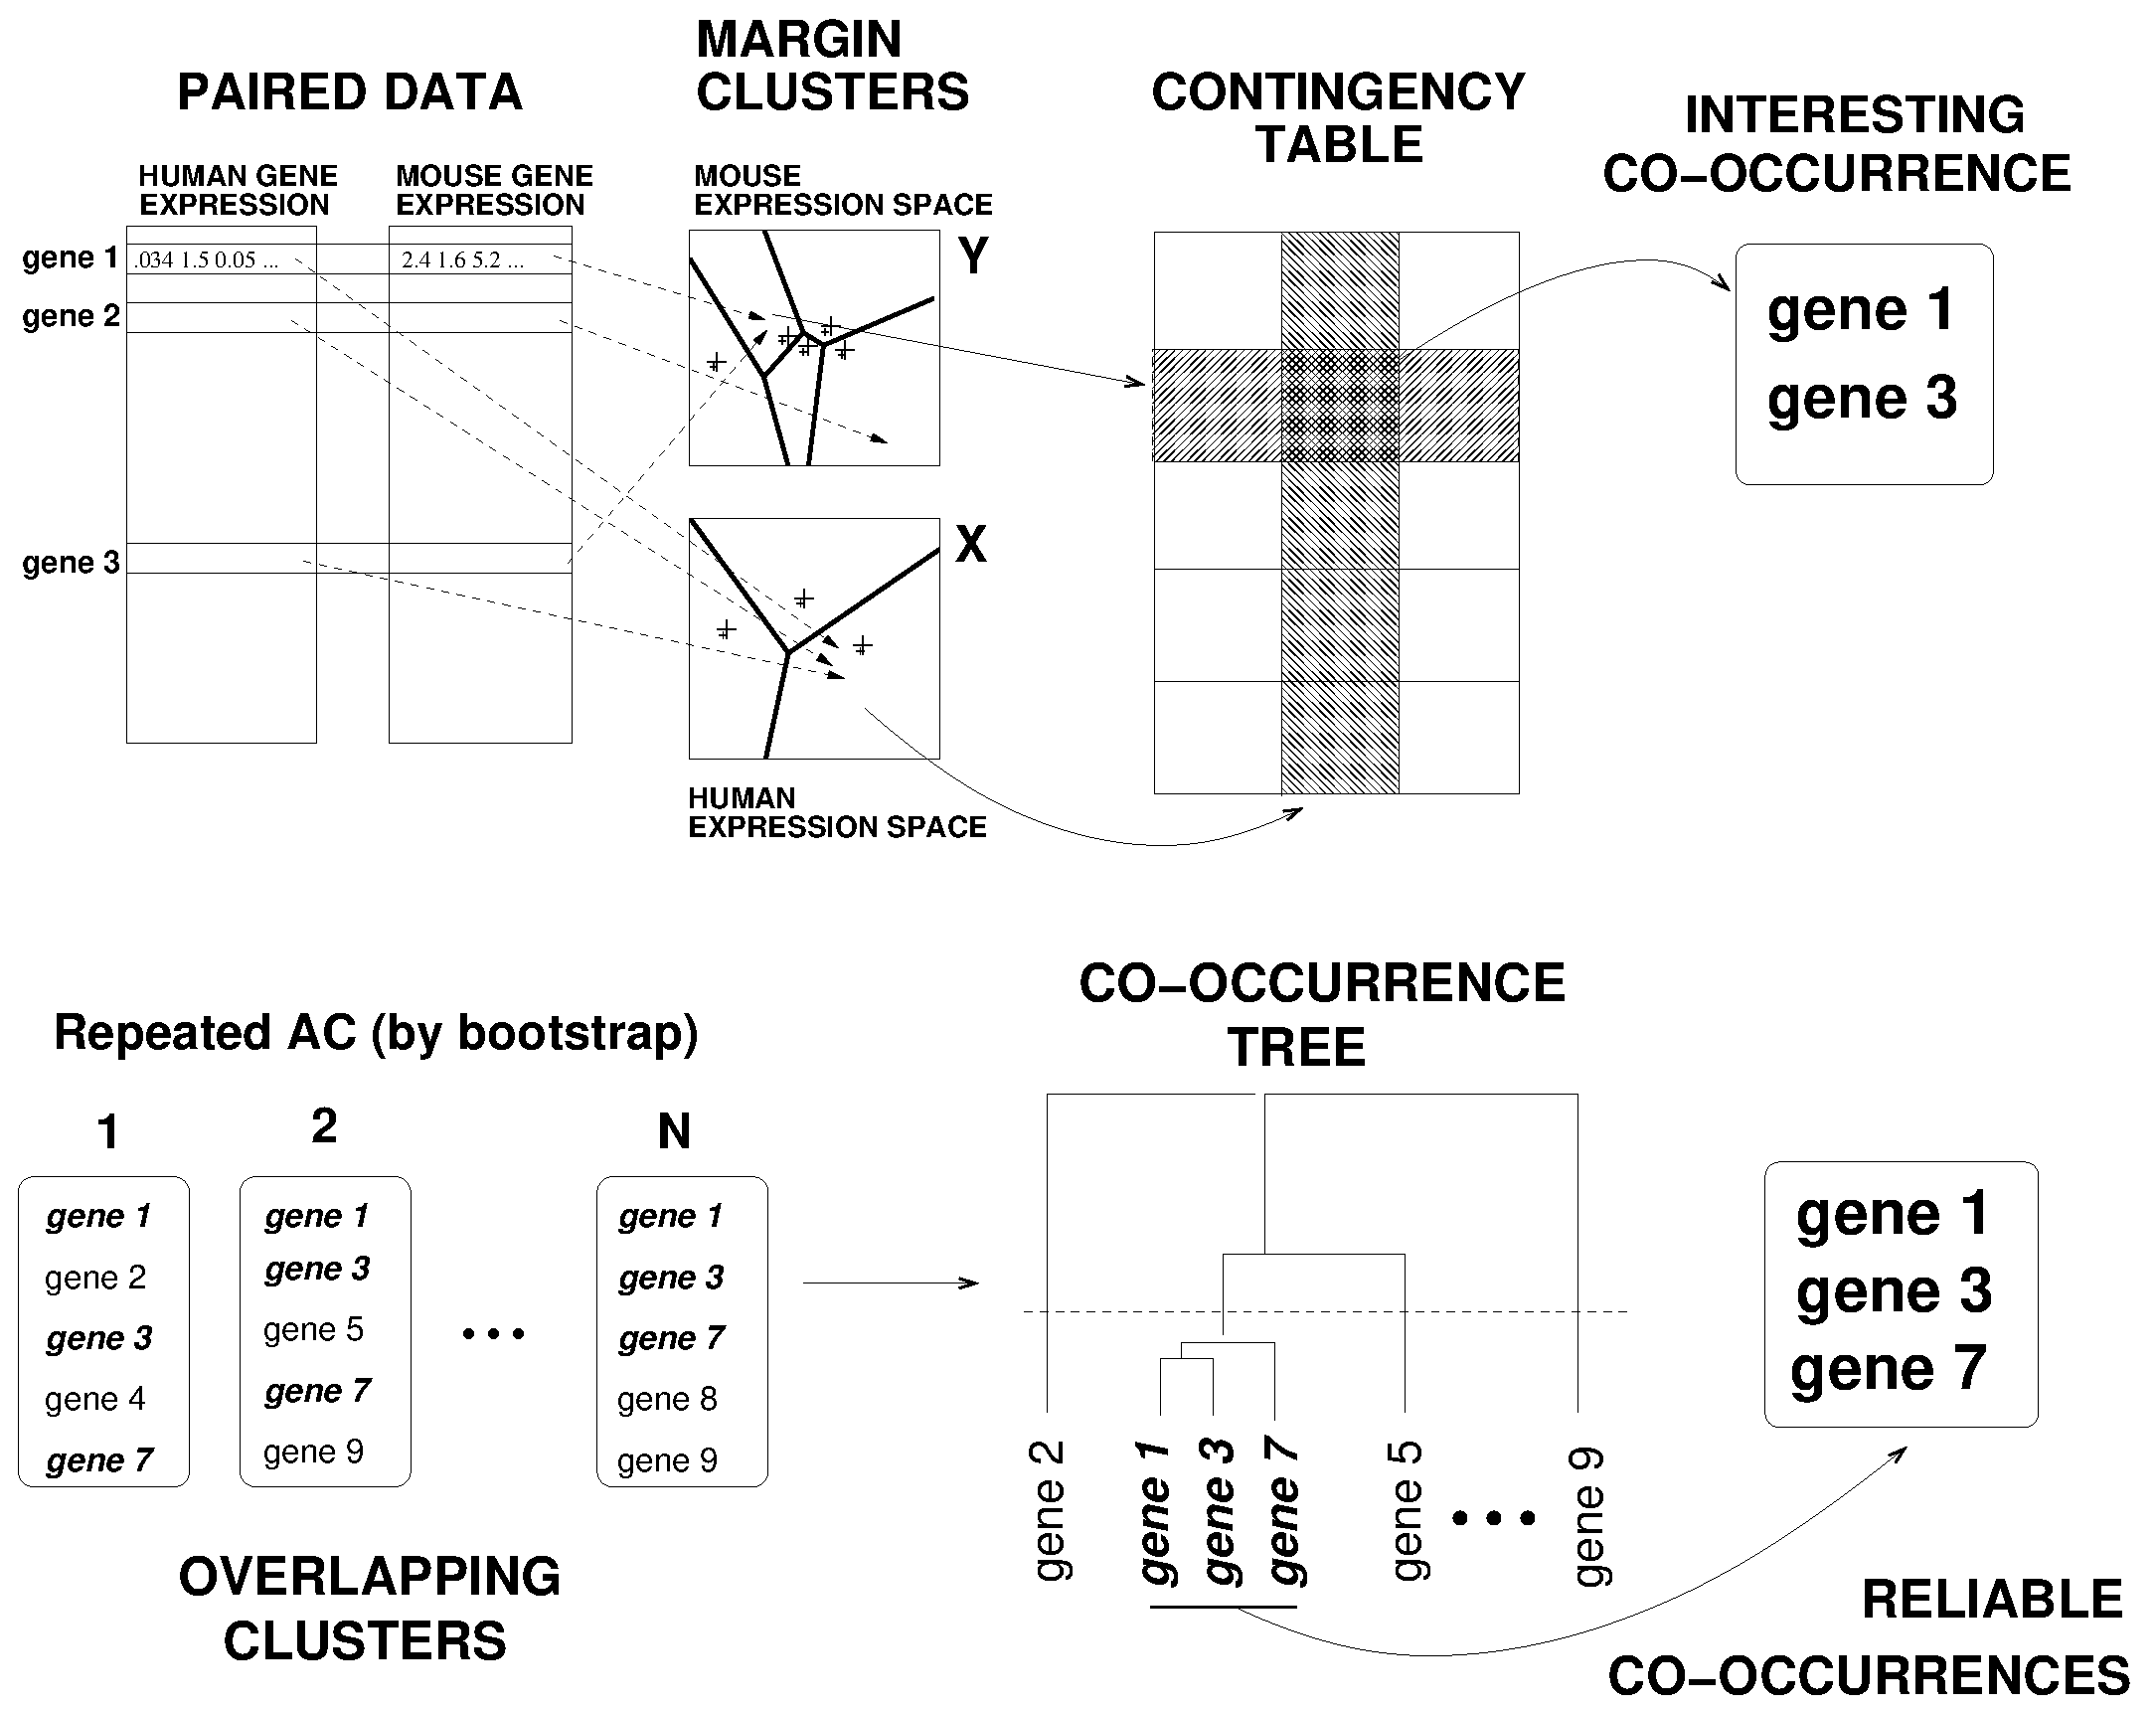
\includegraphics[width=0.9\textwidth]{pic/settingbs.eps}}
\caption{Principle of associative clustering (AC). AC performs
  simultaneous clustering of two data sets, consisting of paired
  observations, and seeks to maximize the dependency between the two
  sets of clusters.  The clusters are defined by cluster centroids in
  each data space.  The clustering results are represented on a
  contingency table, where clusters of the two data sets correspond
  with the rows and columns of the contingency table,
  respectively. These are called the margin clusters of the
  contingency table. The table cells are called cross clusters and
  they contain orthologous genes from the two data sets.  The cluster
  centroids are optimized to produce a contingency table with maximal
  dependency between the margin cluster counts.  Cross clusters that
  show significant deviation from the null hypothesis of independent
  margins indicate dependency. In order to enhance the reliability of
  the results, the clustering is repeated with slightly differing
  bootstrap samples. Then reliable co-occurrences are identified from
  a co-occurrence tree with a specified threshold. Frequently
  co-occurring orthologues are selected for further analyzes.}
\end{figure}

\subsubsection{The associative clustering principle}

The principle of associative clustering (AC) is illustrated in
Figure~\ref{fig:acprinciple}. AC performs simultaneous clustering of
two data sets to reveal maximally dependent cluster structure between
two sets of observations. The clusters are defined in each data space
by {\it Voronoi parameterization}, where the clusters are defined by
cluster centroids to produce connected, internally homogeneous
clusters.  Let us denote the two sets of clusters by
\(\{V^{(x)}_i\}_i\), \(\{V^{(y)}_j\}_j\).  A given data point \(\x\)
is then assigned to the cluster corresponding to the nearest centroid
\(\m_i\) in the feature space, with respect to a given distance
measure\footnote{\(\x \in V_i^{(x)}\) if \(d(\x, \m_i) \leq d(\x,
  \m_k)\) for all \(k\).}  \(d\).  This divides the space into
non-overlapping {\em Voronoi regions}. The regions define a clustering
for all points of the data space. The association between the clusters
of the two data sets can be represented on a contingency table, where
the rows and columns correspond to clusters in the first and second
data set, respectively. The clusters in each data set are called {\it
  margin clusters}. Each pair of co-occurring observations $(\xi,\yi)$
maps to one margin cluster in each data set, and each contingency
table cell corresponds to a pair of margin clusters. These are called
{\it cross clusters}.

AC searches for a maximally dependent cluster structure by optimizing
the Voronoi centroids in the two data spaces in such a way that the
dependency between the contingency table margins is maximized. Let us
denote the number of samples in cross cluster \(i, j\) by
\(n_{ij}\). The corresponding margin cluster counts are $n_{i \cdot} =
\sum_j n_{ij}$ and $n_{\cdot j} = \sum_i n_{ij}$.  The observed sample
frequencies over the contingency table margins and cross-clusters are
assumed to follow multinomial distribution with latent parameters
\(\bth_i, \bth_j\) and \(\bth_{ij}\), respectively.  Assuming the
model $M_I$ of {\it independent margin clusters}, the expected sample
frequency in each cross cluster is given by the outer product of
margin cluster frequencies.  The model $M_d$ of \emph{dependent margin
  clusters} deviates from this assumption. The {\it Bayes factor (BF)}
is used to compare the two hypotheses of dependent and independent
margins. This is a rigorously justified approach for model comparison,
which indicates whether the observations provide superior evidence for
either model. Evidence is calculated over all potential values of the
model parameters, marginalized over the latent frequencies. In a
standard setting, the Bayes factor would be used to compare evidence
between the dependent and independent margin cluster models for a
given clustering solution. AC uses the Bayes factor in a non-standard
manner; as an objective function to maximize by optimizing the cluster
centroids in each data space; the centroids define the margin clusters
and consequently the margin cluster dependencies.

The centroids are optimized with a conjugate-gradient algorithm after
smoothing the cluster borders with continuous parameterization. The
hyperparameters $n^{(d)}$, $n^{(x)}$, and $n^{(y)}$ arise from
Dirichlet priors of the two multinomial models \(M_I\), \(M_D\) of
independent and dependent margins, respectively.  Setting the
hyperparameters to unity yields the classical hypergeometric measure
of contingency table dependency \citep{Fisher34,Yates34}. With large
sample size, the logarithmic Bayes factor approaches mutual
information \citep{Sinkkonen05tr}. The Bayes factor is a desirable
choice especially with a limited sample size since a marginalization
over the latent variables makes it robust against uncertainty in the
parameter values, and because finite contingency table counts would
give a biased estimate of mutual information.  The number of clusters
in each data space is specified in advance, typically based on the
desired level of resolution. Nonparametric extensions, where the
number of margin clusters would be inferred automatically from the
data form one potential topic for further studies; a closely related
approach was recently proposed in \cite{Rogers2010}.

Publication~\ref{AC} introduces an additional, bootstrap-based
procedure to assess the reliability of the findings
(Figure~\ref{fig:acprinciple}). The analysis is repeated with similar,
but not identical training data sets obtained by sampling the original
data with replacement. The most frequently detected dependencies are
then investigated more closely. The analysis will emphasize findings
that are not sensitive to small variations in the observed data.

\subsubsection{Comparison methods}

Associative clustering was compared with two alternative methods:
standard K-means on each of the two data sets, and a combination of
K-means and information bottleneck (K-IB). K-means \citep[see
e.g.][]{Bishop06} is a classical clustering algorithm that provides
homogeneous, connected clusters based on Voronoi
parameterization. Homogeneity is desirable for interpretation, since
the data points within a given cluster can then be conveniently
summarized by the cluster centroid. On the other hand, K-means
considers each data set independently, which is suboptimal for the
dependency modeling task. The two sets of clusters obtained by
K-means, one for each data space, can then be presented on a
contingency table as in associative clustering.  The second comparison
method is K-IB introduced in Publication~\ref{ECML}. K-IB uses K-means
to partition the two co-occurring, continuous-valued data sets into
discrete atomic regions where each data point is assigned in its own
singleton cluster. This gives two sets of atomic clusters that are
mapped on a large contingency table, filled with frequencies of
co-occurring data pairs $(\x_k, \y_k)$. The table is then compressed
to the desired size by aggregating the margin clusters with the
symmetric IB algorithm in order to maximize the dependency between the
contingency table margins \citep{Friedman01}.  Aggregating the atomic
clusters provides a flexible clustering approach, but the resulting
clusters are not necessarily homogeneous and they are therefore
difficult to interpret.

AC compared favorably to the other methods.  While AC outperformed the
standard K-means in dependency modeling, the cluster homogeneity was
not significantly reduced in AC. The cross clusters from K-IB
\citep{Sinkkonen03tr} were more dependent than in AC. On the other
hand, AC produced more easily interpretable localized clusters, as
measured by the sum of intra-cluster variances in
Publication~\ref{AC}. Homogeneity makes it possible to summarize
clusters conveniently, for instance by using the mean expression
profiles of the cluster samples, as in Figure~\ref{fig:ctable}B.
While K-means searches for maximally homogeneous clusters and K-IB
searches for maximally dependent clusters, AC finds a successful
compromise between the goals of dependency and homogeneity.

\begin{figure}[t]
\centerline{
\begin{tabular}{cc}
{\bf A}&{\bf B}\\
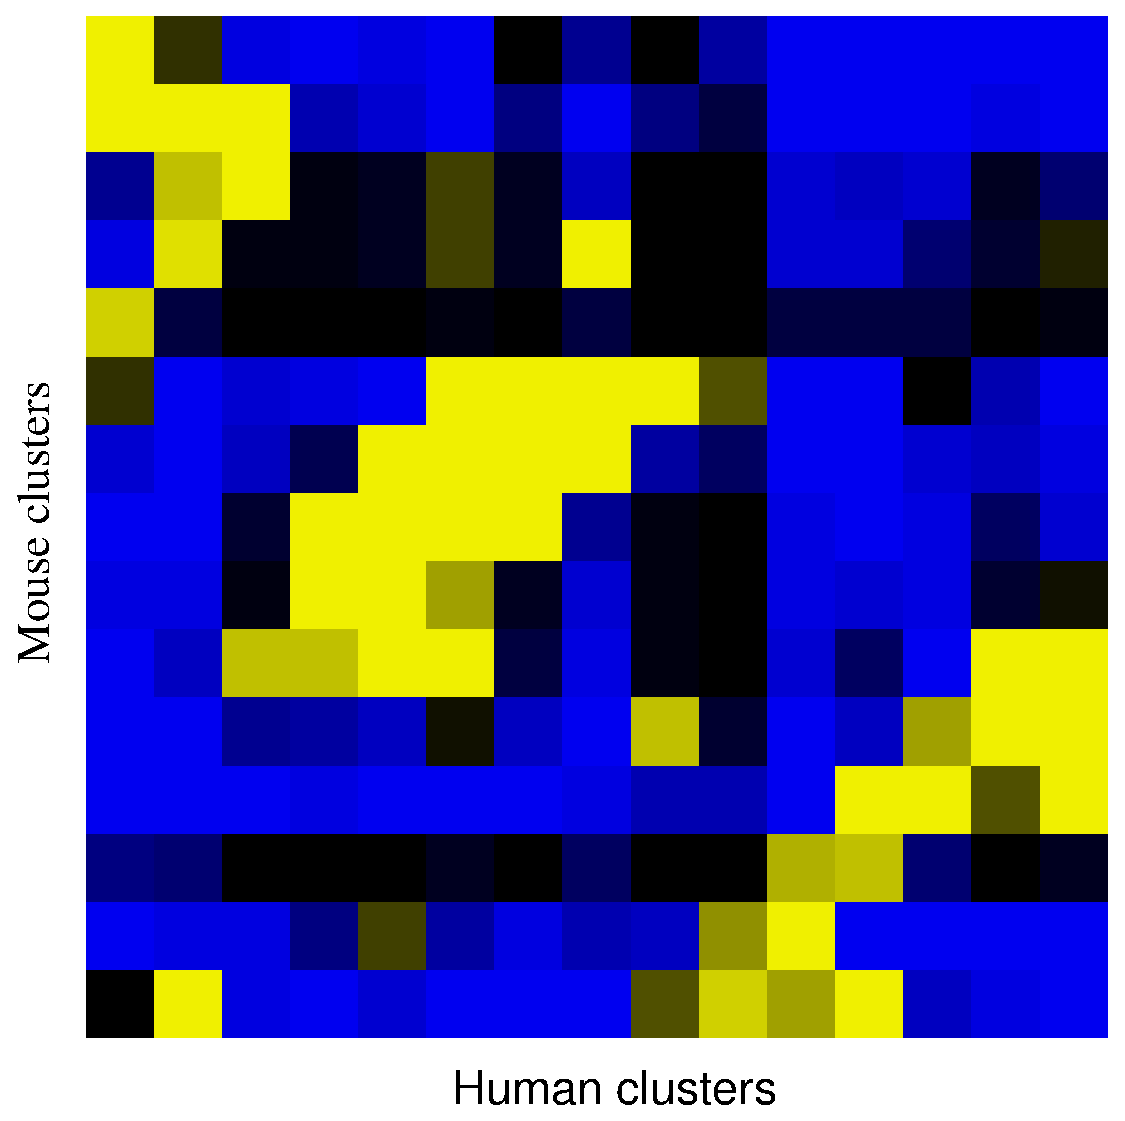
\includegraphics[width=0.4\textwidth]{pic/ctable.eps}& 
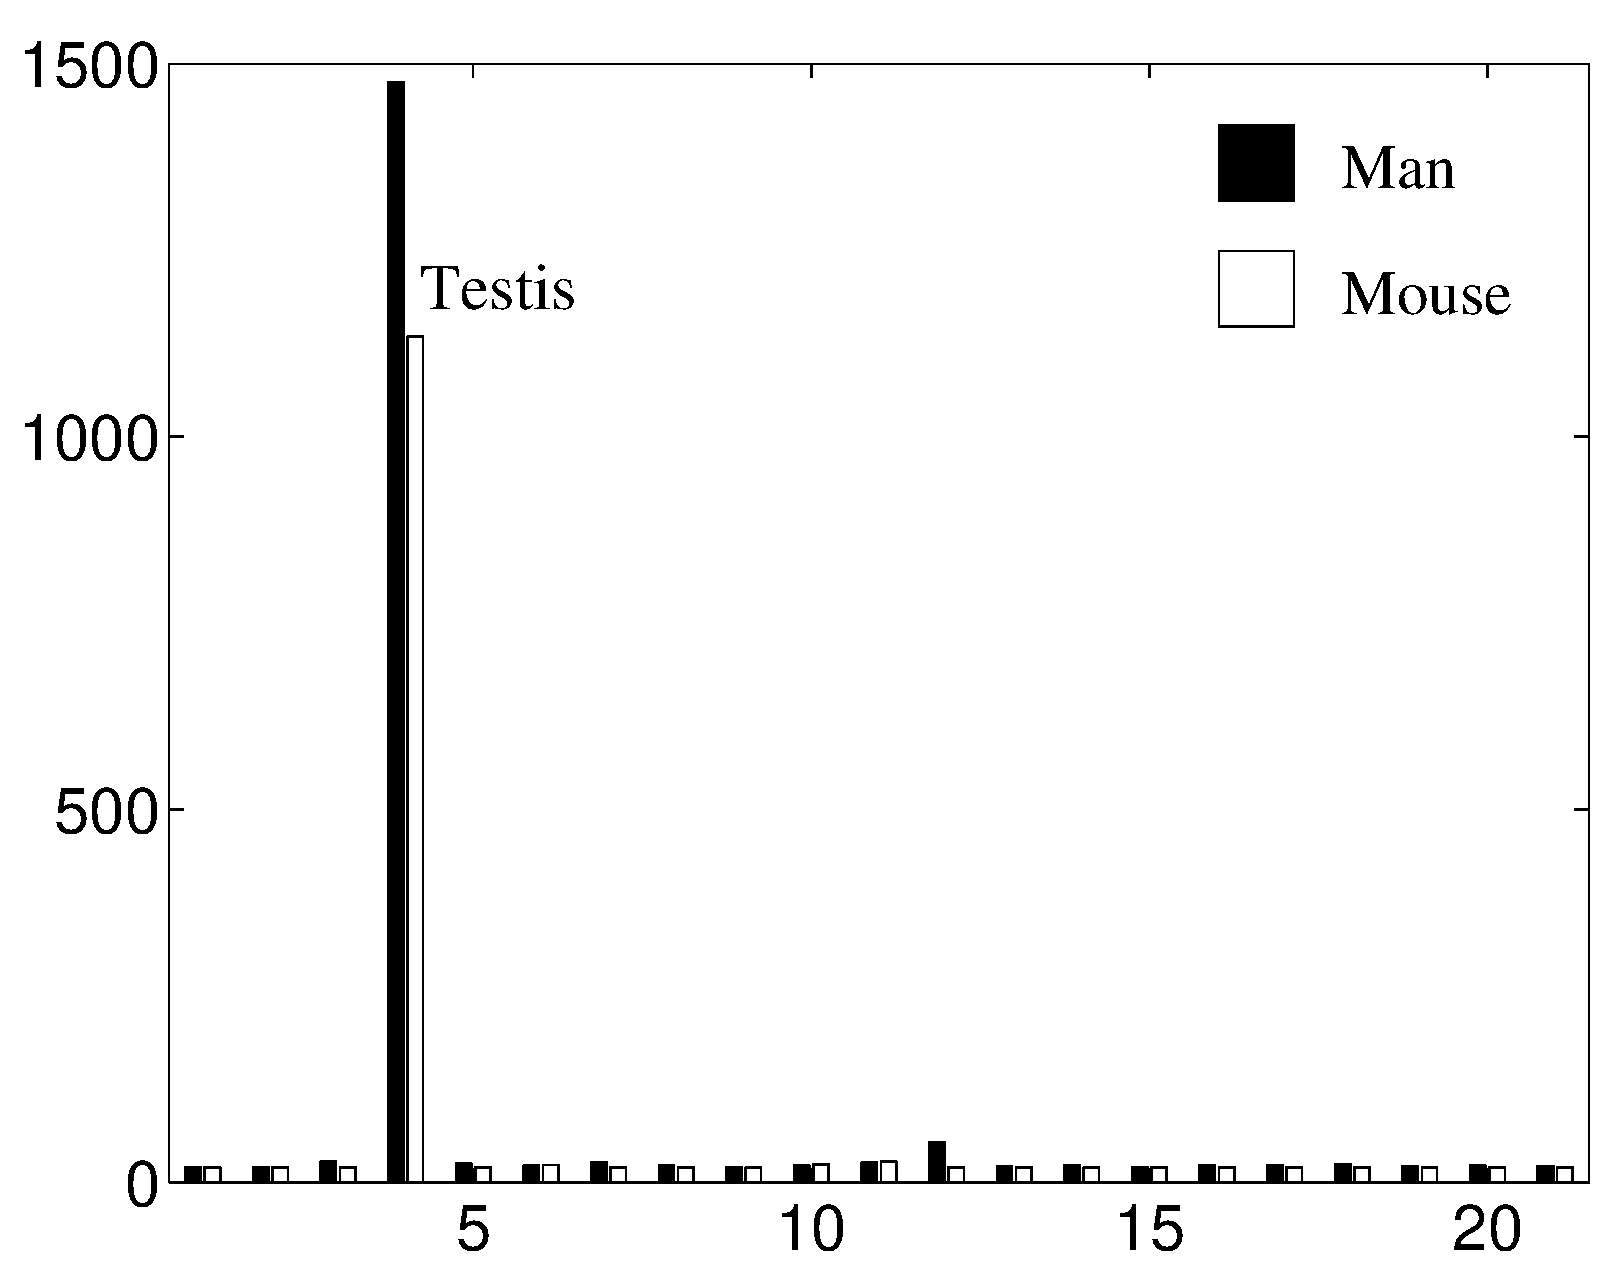
\includegraphics[width=0.5\textwidth]{pic/testis.eps}
\end{tabular}
}
\caption{{\bf A} The contingency table of associative clustering
  highlights orthologous gene groups in human (rows) and mouse
  (columns) with exceptional levels of conservation (yellow) or
  divergence (blue) in transcriptional activity between the two
  species. {\bf B} Average expression profiles of a highly conserved
  group of testis-specific genes across 21 tissues in man and
  mouse. \copyright IEEE. Reprinted with permission from
  Publication~\ref{AC}.}
\label{fig:ctable}
\end{figure}
%/share/mi/mi/papers/bioinf_conf04/manmouse/pic



\subsection{Exploratory analysis of transcriptional divergence between
  species}

Associative clustering is used in Publications~\ref{ECML} and~\ref{AC}
to investigate conservation and divergence of transcriptional activity
of 2818 orthologous human-mouse gene pairs across an organism-wide
collection of transcriptional profiling data covering 46 and 45 tissue
types in human and mouse, respectively \citep{Su02}. AC takes as input
two gene expression matrices with orthologous genes, one for each
species, and returns a dependency-maximizing clustering for the
orthologous gene pairs.  Interpretation of the results focuses on
unexpectedly large or small cross clusters revealed by the contingency
table analysis of associative clustering. Compared to plain
correlation-based comparisons between the gene expression profiles, AC
can reveal additional cluster structure, where genes with similar
expression profiles are clustered together, and associations between
the two species are investigated at the level of such detected gene
groups. The dependency between each pair of margin clusters can be
characterized by comparing the respective margin cluster centroids
that provide a compact summary of the samples within each cluster.

Biological interpretation of the findings, based on enrichment of Gene
Ontology (GO) categories \citep{Ashburner00}, revealed genes with
strongly conserved and potentially diverged transcriptional
activity. The most highly enriched categories were associated with
ribosomal functions, the high conservation of which has also been
suggested in earlier studies \citep{Jimenez02}; ribosomal genes often
require coordinated effort of a large group of genes, and they
function in cell maintenance tasks that are critical for species
survival.  An exceptional level of conservation was also observed in a
group of testis-specific genes, yielding novel functional hypotheses
for certain poorly annotated genes within the same cross-cluster
(Figure~\ref{fig:ctable}). Transcriptional divergence, on the other
hand, was detected for instance in genes related to embryonic
development.

While general-purpose dependency exploration tools may not be optimal
for studying the specific issue of transcriptional conservation, such
tools can reveal dependency with minimal prior knowledge about the
data. This is useful in functional genomics experiments where little
prior knowledge is available. In Publications~\ref{ECML} and~\ref{AC},
associative clustering has been additionally applied in investigating
dependencies between transcriptional activity and transcription factor
binding, another key regulatory mechanism of the genes.


\section{Conclusion}

The models introduced in Publications~\ref{MLSP}-\ref{AC} provide
general exploratory tools for the discovery and analysis of
statistical dependencies between co-occurring data sources and tools
to guide modeling through Bayesian priors. In particular, the models
consider linear dependencies (Publication~\ref{MLSP}) and
cluster-based dependency structures (Publications~\ref{ECML}-\ref{AC})
between the data sources. The models are readily applicable to data
integration tasks in functional genomics. In particular, the models
have been applied to investigate dependencies between chromosomal
mutations and transcriptional activity in cancer, and evolutionary
divergence of transcriptional activity between human and mouse.
Biomedical studies provide a number of other potential applications
for such general-purpose methods. An increasing number of co-occurring
observations across the various regulatory layers of the genome are
available concerning epigenetic mechanisms, micro-RNAs, polymorphisms
and other genomic features \citep{tcga08}. Simultaneous observations
provide a valuable resource for investigating the functional
properties that emerge from the interactions between the different
layers of genomic information. An open source implementation in
BioConductor\footnote{http://www.bioconductor.org/packages/release/bioc/html/pint.html}
provides accessible computational tools for related data integration
tasks, helping to guarantee the utility of the developed models for
the computational biology community.

